\documentclass[11pt, english]{article}
\usepackage{graphicx}
\usepackage[colorlinks=true, linkcolor=blue]{hyperref}
\usepackage[english]{babel}
\selectlanguage{english}
\usepackage[utf8]{inputenc}
\usepackage[svgnames]{xcolor}
\usepackage{svg}

\usepackage{listings}
\usepackage{afterpage}
\pagestyle{plain}

\definecolor{dkgreen}{rgb}{0,0.6,0}
\definecolor{gray}{rgb}{0.5,0.5,0.5}
\definecolor{mauve}{rgb}{0.58,0,0.82}

\renewcommand{\lstlistingname}{Ejemplo}% Listing -> Ejemplo

\lstdefinestyle{customc}{
  numbers=left,
  belowcaptionskip=1\baselineskip,
  breaklines=true,
  frame=L,
  xleftmargin=\parindent,
  language=C,
  showstringspaces=false,
  basicstyle=\footnotesize\ttfamily,
  keywordstyle=\bfseries\color{green!40!black},
  commentstyle=\itshape\color{purple!40!black},
  identifierstyle=\color{blue},
  stringstyle=\color{orange},
}

%\lstset{language=R,
%    basicstyle=\small\ttfamily,
%   stringstyle=\color{DarkGreen},
%    otherkeywords={0,1,2,3,4,5,6,7,8,9},
%    morekeywords={TRUE,FALSE},
%    deletekeywords={data,frame,length,as,character},
%    keywordstyle=\color{blue},
%    commentstyle=\color{DarkGreen},
%}

\lstset{frame=tb,
language=R,
aboveskip=3mm,
belowskip=3mm,
showstringspaces=false,
columns=flexible,
numbers=none,
keywordstyle=\color{blue},
numberstyle=\tiny\color{gray},
commentstyle=\color{dkgreen},
stringstyle=\color{mauve},
breaklines=true,
breakatwhitespace=true,
tabsize=3
}

\usepackage{here}


\textheight=21cm
\textwidth=17cm
%\topmargin=-1cm
\oddsidemargin=0cm
\parindent=0mm
\pagestyle{plain}

%%%%%%%%%%%%%%%%%%%%%%%%%%
% La siguiente instrucción pone el curso automáticamente%
%%%%%%%%%%%%%%%%%%%%%%%%%%

\usepackage{color}
\usepackage{ragged2e}

\global\let\date\relax
\newcounter{unomenos}
\setcounter{unomenos}{\number\year}
\addtocounter{unomenos}{-1}
\stepcounter{unomenos}
\gdef\@date{ Course \arabic{unomenos}/ 2019}

\begin{document}

\begin{titlepage}

\begin{center}
\vspace*{-1in}
\begin{figure}[htb]
\begin{center}
\centering
\begin{tabular}{@{}cccc@{}}

\includegraphics[width=6cm]{images/EscudoUNAM.png}
\hspace*{1.2in}

\includegraphics[width=6cm]{images/logoIng.png}
\end{tabular}
\end{center}
\end{figure}

FACULTAD DE INGENIERÍA - \@date\\
\vspace*{0.15in}
SECRETARÍA/DIVISIÓN: DIVISIÓN DE INGENIERÍA ELÉCTRICA \\
ÁREA/DEPARTAMENTO: INGENIERÍA EN COMPUTACIÓN \\
\vspace*{0.4in}
\begin{large}
LABORATORIO DE COMPUTACIÓN GRÁFICA E INTERACCIÓN HUMANO COMPUTADORA:\\
\end{large}
\vspace*{0.2in}
\begin{Large}
\textbf{Proyecciones y puertos de vista. Transformaciones Geométricas } \\
\end{Large}
\vspace*{0.3in}
\vspace*{0.3in}
\begin{large}
Reynaldo Martell Avila \\
\end{large}
\vspace*{0.5in}
\vspace*{0.5in}
\begin{large}
\textbf{PRÁCTICA 3} \\
\end{large}
\end{center}
\end{titlepage}

\newcommand{\CC}{C\nolinebreak\hspace{-.05em}\raisebox{.4ex}{\tiny\bf +}\nolinebreak\hspace{-.10em}\raisebox{.4ex}{\tiny\bf +}}
\def\CC{{C\nolinebreak[4]\hspace{-.05em}\raisebox{.4ex}{\tiny\bf ++}}}

\tableofcontents

\newpage
\section{Objetivos de aprendizaje}
\subsection{Objetivos generales:}
El alumno repasará como crear buffers de OpenGL, leer archivos, comprenderá los
diferentes tipos de proyección y las funciones de la librería glm para crear éstas, así como
comprenderá los diferentes sistemas de referencia de OpenGL. Del mismo modo practicará
como colocar en la escena diferentes geometrías.
\subsection{Objetivos específicos:}
El alumno practicará crear geometrías con índices, revisará los sistemas de referencia que
se aplican en OpenGL, comprenderá la utilización de la matriz de modelo, vista, proyección
y la zona de dibujo.
\section{Recursos a emplear}
\subsection{Software}
Sistema Operativo: Windows 7
Ambiente de Desarrollo: Visual Studio 2017.
\subsection{Equipos}
Los equipos de cómputo con los que cuenta el laboratorio de Computación Gráfica
\subsection{Instrumentos}
\section{Fundamento Teórico}
\begin{itemize}
\item \textbf{Presentación de conceptos.} \\
Se mostrará la utilización de índices, se revisará como crear los shaders de fragmento y
vértices desde un archivo, se presentará el funcionamiento de variables globales que son
tomadas de los shaders, utilizará los diferentes tipos de proyecciones y funciones para
crearlas, así como colocar diferentes figuras en pantalla.
\item \textbf{Datos necesarios.}
Librería OpenGL 3.3, librería de creación de ventanas, IDE de desarrollo (Visual Studio 2017.
\end{itemize}
\subsection{Desarrollo de actividades}
\begin{enumerate}
\item Ejecutar el código base de la práctica \textbf{03-SistemasCoordenados}, observar la ejecución.
\item Explicar el código de la Clase \textbf{Shader.h} y su implementación \textbf{Shader.cpp}.
\item Utilice la Clase Shader para instanciar un objeto de éste tipo, para utilizarlo es necesario incluir  la cabecera \textbf{\#include "Headers/Shader.h"}, para instanciar el objeto utilice: \textbf{Shader shader;} y por último agregar la inicialización de los shaders en el método initialize: \textbf{shader.initialize("../Shaders/transformaciones.vs", "../Shaders/transformaciones.fs");}
\item Localizar y abrir los archivo que contienen el código de los Shaders \textbf{../Shaders/transformaciones.vs} y \textbf{../Shaders/transformaciones.fs}.
\item Se explican los código de los Shaders.
\item Crear una matriz de proyección en perspectiva en el loop principal: \\ \textbf{glm::mat4 projection = glm::perspective(glm::radians(45.0f), (float) screenWidth / (float) screenHeight, 0.01f, 100.0f);}
\item Agregar la matriz de modelo vista y proyección, realizar una translación a la matriz de vista en dirección del vector $\bar{v} = (0.0, 0.0, -3.0)$,y por ulimo enviar las matrices a los shaders. Tomar como ejemplo el código de la sección \ref{list:first}.

\begin{lstlisting}[label={list:first},caption={Ejemplo para envíar las matrices del modelo, vista y proyección.}, style=customc]
glm::mat4 model = glm::mat4(1.0f);
glm::mat4 view = glm::mat4(1.0f);
view = glm::translate(view, glm::vec3(0.0f, 0.0f, -3.0f));

shader.setMatrix4("model", 1, false, glm::value_ptr(model));
shader.setMatrix4("view", 1, false, glm::value_ptr(view));
shader.setMatrix4("projection", 1, false, glm::value_ptr(projection));
\end{lstlisting}

\item Agregar la bandera \textbf{GL\_DEPTH\_BUFFER\_BIT} a la función \textbf{glClear}, con esta bandera se refrescan el buffer de color y el buffer de profundidad.\\ \textbf{glClear(GL\_COLOR\_BUFFER\_BIT $\mid$ GL\_DEPTH\_BUFFER\_BIT);}, despúes de esta línea de código agregar la activación del shader \textbf{shader.turnOn();}, esta función se encarga de indicar que programa usar, es equivalente a \textbf{glUseProgram(shaderProgramID);}.

\item Ejecutar el programa y revisar sí la geometría corresponde a la especificada en el arreglo.

\item Crear otro buffer de tipo \textbf{GL\_ELEMENT\_ARRAY\_BUFFER}.
\begin{lstlisting}[label={list:second},caption={Ejemplo para crear un arreglo de indices.}, style=customc]
// Cambiamos el estado para indicar que usaremos el id del EBO como Arreglo de indices (GL_ELEMENT_ARRAY_BUFFER)
glBindBuffer(GL_ELEMENT_ARRAY_BUFFER, EBO);
// Copiamos los datos de los vertices a memoria del procesador grafico
//           TIPO DE BUFFER     TAMANIO          DATOS    MODO (No cambian los datos)
glBufferData(GL_ELEMENT_ARRAY_BUFFER, sizeof(indices), indices, GL_STATIC_DRAW);
\end{lstlisting}

 En éste se almacenará el arreglo \textbf{indices}, el arreglo indices indica la conexión de cada vertice, ésto ahorra la cantidad de memoria que se ocupa, aún que por otro lado se requiere un arreglo de enteros. Remplazar la función \textbf{glDrawArrays(GL\_TRIANGLES, 0, 3);} por \textbf{glDrawElements(GL\_TRIANGLES, 24, GL\_UNSIGNED\_INT, 0);}

\item Cambiar el sistema de referencia de puerto de vista con la función \textbf{glViweport(GLint x, GLint y, GLsizei width, GLsizei height)}:
\begin{itemize}
\item x, y: Son las coordenadas de la esquina inferior izquierda de la zona de dibujo
\item width, height: Especifican el ancho y alto de la zona de dibujo.
\end{itemize}

Probar con los siguientes parámetros:

\begin{itemize}
\item Dividir a la mitad la zona de dibujo en el eje y.
\item La esquina inferior en las coordenadas (0, 0) y el tamaño de la zona de dibujo a la mitad de cada eje.
\end{itemize}

\item Colocar dos cubos en dos diferentes posiciones y diferente profundidad en z, ejemplo 

\begin{lstlisting}[label={list:third},caption={Ejemplo para colocar dos cubos.}, style=customc]
shader.turnOn();

glm::mat4 view = glm::mat4(1.0f);
view = glm::translate(view, glm::vec3(0.0f, 0.0f, -3.0f));

shader.setMatrix4("view", 1, false, glm::value_ptr(view));
shader.setMatrix4("projection", 1, false, glm::value_ptr(projection));

glm::mat4 model = glm::translate(glm::mat4(1.0), glm::vec3(-1.0, 1.0, -2.0));
shader.setMatrix4("model", 1, false, glm::value_ptr(model));

// Se indica el buffer de datos y la estructura de estos utilizando solo el id del VAO
glBindVertexArray(VAO);
// Primitiva de ensamble
glDrawElements(GL_TRIANGLES, 24, GL_UNSIGNED_INT, 0);
glBindVertexArray(0);

model = glm::translate(glm::mat4(1.0), glm::vec3(2.0, 1.0, -4.0));
shader.setMatrix4("model", 1, false, glm::value_ptr(model));

// Se indica el buffer de datos y la estructura de estos utilizando solo el id del VAO
glBindVertexArray(VAO);
// Primitiva de ensamble
glDrawElements(GL_TRIANGLES, 24, GL_UNSIGNED_INT, 0);
glBindVertexArray(0);

shader.turnOff();
\end{lstlisting}

\item Se explica y se cambian los parámetros que definen los diferentes tipos de
proyecciones.

\begin{itemize}
\item \textbf{glm::mat4 projection = glm::perspective(glm::radians(45.0f), (float) screenWidth / (float) screenHeight, 0.01f, 100.0f);}
\item \textbf{glm::mat4 projection = glm::frustum(-0.005, 0.005, -0.005, 0.005, 0.01, 100.0);}
\item \textbf{glm::mat4 projection = glm::ortho(-5.0, 5.0, -5.0, 5.0, 0.01, 10.0);}
\end{itemize}
\end{enumerate}

\subsection{Ejercicios}
\begin{enumerate}
\item Los siguientes ejercicios se deben crear con un cubo con un color por cada lado. Se debe crear otro VAO y VBO
\item Utilizando un cubo unitario con centro en el origen como primitiva, y la
transformación de translación y escalamiento, se creará una escena con las siglas CG 2019.

\item Se procede a crear un par de figuras instanciado el cubo y aplicando
transformaciones básicas a cada una de las instancias.
\begin{figure}[htb]
\begin{center}
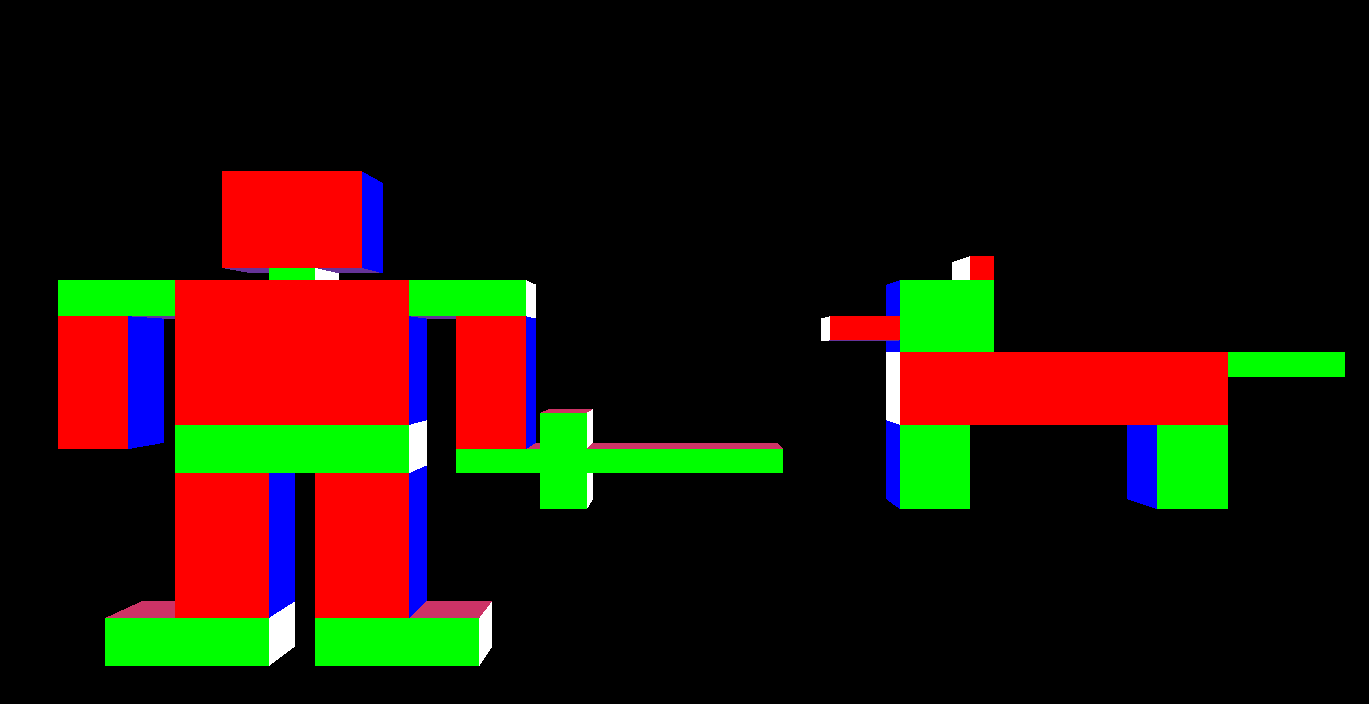
\includegraphics[width=10cm]{images/Transformaciones.png}
\end{center}
\end{figure}
\item Crear la misma forma de la estrella de la práctica 2 con indices.
\item Deben subir sus ejercicios en Github y colocar la liga en su reporte.
\end{enumerate}
\section{Observaciones y Conclusiones}
\section{Anexos}
\begin{enumerate}
\item Cuestionario previo.
\begin{enumerate}
\item ¿Qué es una clase en c++?
\item ¿Qué es un constructor y destructor de la clase, y cómo se declara en
c++?
\item ¿Cómo se instancia un objeto en c++?
\item Investigar como abrir un archivo en c++.
\item Investigue para qué sirve la función \textbf{glViewport} y que parámetros
recibe.
\item Investigue que es la matriz de Modelo, Vista, Proyección.
\item ¿Qué es una proyección e investigue los tipos de proyecciones, en el
ámbito de gráficos?
\item Que utilidad tiene las funciones \textbf{glm::ortho}, \textbf{glm::frustum} y
\textbf{glm::perspective}, y que son los parámetros que reciben.
\item Para qué sirve la función \textbf{glfwSetWindowPos} y que parámetros recibe.
\item ¿Cuáles son las transformaciones geométricas básicas en tres
dimensiones y sus matrices asociadas?
\item Investigué para sirve la función \textbf{glm::scale}, \textbf{glm::translate}, \textbf{glm::rotate},
y que parámetros reciben.
\end{enumerate}
\item Actividad de investigación previa.
\begin{enumerate}
\item Realizar un \textbf{git pull origin master} y un \textbf{git pull myRepo master}, antes de comenzar la práctica.
\end{enumerate}
\end{enumerate}

%uoooooooooooooooo tumadreuooooooooooooooooooo UOOOOOOOOOOOOOOOOOOOOOOOOOOOOOOOOOOOOOOOOO
%AL FIN SE TERMINA ESTA PUTA MIERDA!!!!
%USEGREAS OSTOJEOGIRN ojeogiek


\end{document}